% !TEX encoding = UTF-8
% !TEX TS-program = pdflatex
% !TEX root = ../tesi.tex

%**************************************************************
\chapter{Descrizione dello stage}
\label{cap:descrizione-stage}
%**************************************************************

\intro{Breve introduzione al capitolo}\\

In questo capitolo viene descritto come si è pianificato e svolto lo stage presso SAI, introducendo il progetto, considerando gli obiettivi e i possibili rischi.

%**************************************************************
\section{Introduzione al progetto}

o stage svolto presso SAI aveva come scopo la creazione di un prototipo di piattaforma web/desktop per il caricamento delle registrazioni audio effettuate nelle aule di tribunale, con l'aiuto di alcuni metadata prodotti durante le medesime registrazioni. In particolare l'applicazione da sviluppare è divisa in due parti backend e frontend (spiegare meglio back e front) che comunicano tra loro mediante API rest (spiegare API). Lo stage si è focalizzato sullo sviluppo della parte frontend, avanzando di pari passo con lo sviluppo del  backend realizzata da altri membri del team di sviluppo. Per la realizzazione del frontend si è scelto di utilizzare Javascript con i framework React e Redux.

%**************************************************************
\section{Analisi preventiva dei rischi}

Nella fase di analisi iniziali si sono individuati i principali rischi a cui si poteva andare incontro e si è proceduto a definire le possibili soluzione per farne fronte.\\

\begin{risk}{Uso di nuove tecnologie}
  \riskdescription{le tecnologie proposte per la gestione e lo sviluppo del progetto erano per lo più nuove o scarsamente conosciute.}
  \risksolution{è stato previsto un periodo iniziale di studio e formazione su queste tecnologie.}
  \label{risk:new-tecnology}
\end{risk}
\begin{risk}{Modalità di lavoro smart working}
  \riskdescription{lo stage è stato fatto completamente da remoto, e poteva portare ad una possibile mancanza di comunicazione e ad un incertezza nelle attività da svolgere.}
  \risksolution{il tutor aziendale si è reso disponibile a vari meeting nelle prime fasi del progetto e nella formazione iniziale, e rimanendo a disposizione per altri meeting  in caso di dubbi sulle attività da svolgere.}
  \label{risk:smart-working}
\end{risk}

%**************************************************************
\section{Requisiti e obiettivi}

Si farà riferimento ai requisiti secondo le seguenti notazioni:
\begin{itemize}
  \item O per i requisiti obbligatori, vincolanti in quanto obiettivo primario richiesto dal committente;
  \item D per i requisiti desiderabili, non vincolanti o strettamente necessari, ma dal riconoscibile valore aggiunto;
  \item F per i requisiti facoltativi, rappresentanti valore aggiunto non strettamente competitivo.
        Le sigle precedentemente indicate saranno seguite da una coppia sequenziale di numeri, identificativo del requisito.
\end{itemize}

\begin{center}
  \renewcommand{\arraystretch}{1.8} %aumento ampiezza righe
  \begin{tabular}{ |l|l| }
    %    \caption{Tabella del tracciamento dei requisti dello stage}
    %    \label{tab:requisiti-stage}
    \hline
    \textbf{Codice} & \textbf{Descrizione}                                                                \\
    \hline
    O01             & autenticazione mediante server remoto                                               \\
    \hline
    O02             & lettura dati da CD                                                                  \\
    \hline
    O03             & precompilazione di form con i dati caricati da CD                                   \\
    \hline
    O04             & editing dei dati del form                                                           \\
    \hline
    D01             & upload dei dati verso i sistemi esterni                                             \\
    \hline
    D02             & test di unità esaustivi                                                             \\
    \hline
    F01             & possibilità di ascoltare le registrazioni                                           \\
    \hline
    F02             & possibilità di modificare i dati mediante interazioni evolute (per es. drag-n-drop) \\
    \hline
    F03             & realizzazione di un'applicazione desktop con Electron                               \\
    \hline
    F04             & compilazione multipiattaforma dell'applicazione desktop                             \\
    \hline
  \end{tabular}
\end{center}

%**************************************************************
\section{Pianificazione}

La pianificazione, in termini di quantità di ore, sarà distribuita in attività di studio e attività implementative.

Lo stage è stato strutturato in due fasi principali, la prima dedicata alle attività di studio e la seconda alle attività implementative. Di seguito vengono elencate le attività pianificate con la relativa quantità di ore stimata per ogni attività.

\begin{itemize}
  \item Studio delle tecnologie (80 ore)
        \begin{itemize}
          \item Setup di un prototipo di applicazione React e del backend (16 ore);
          \item Studio delle librerie necessarie (React, Redux, JWT, OAuth) (64 ore);
        \end{itemize}
  \item Implementazione prototipo (240 ore)
        \begin{itemize}
          \item Realizzazione dell’interfaccia di login (30 ore);
          \item Implementazione lettura e visualizzazione dei dati da CD (70 ore);
          \item Implementazione editing dei dati letti da CD (70 ore);
          \item Implementazione upload dei dati (30 ore);
          \item Testing dei prodotti realizzati (40ore);
        \end{itemize}
\end{itemize}

Per ogni attività riguardante la fase di implementazione del prototipo è stata prevista anche la relativa attività di testing.
Il tutto viene rappresentato dal seguente dal diagramma di Gantt.
\begin{center}
  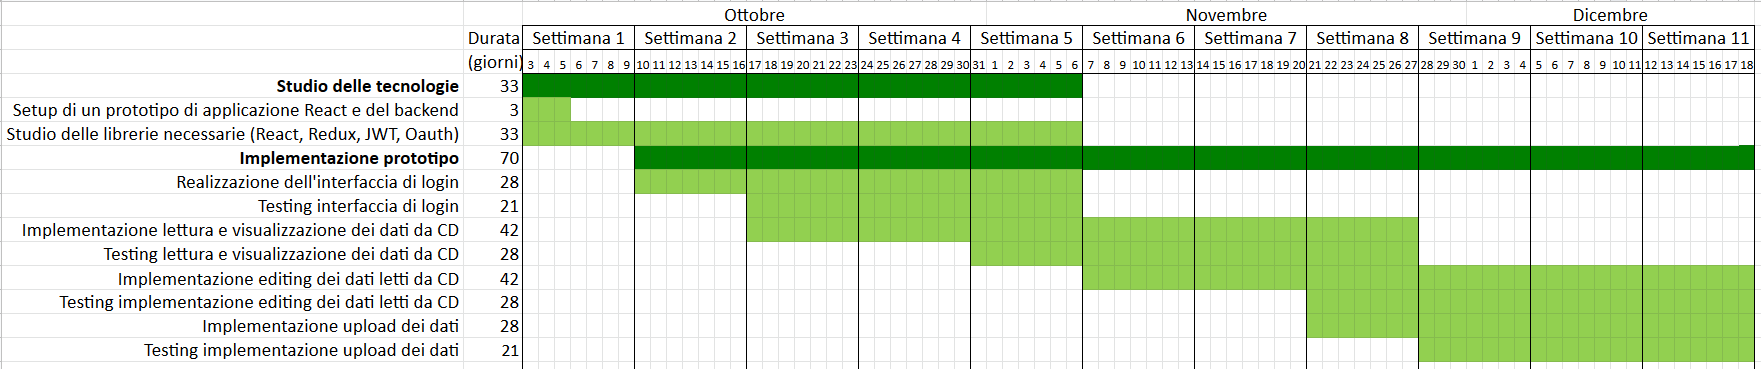
\includegraphics[width=14cm]{gantt}
\end{center}

%**************************************************************
\section{Strumenti}

L'azienda usa un'infrastruttura già collaudata della quale fanno parte sistemi di versionamento del codice, strumenti per l'organizzazione del lavoro e per la comunicazione all'interno del gruppo di lavoro.
Di suguito una panoramica dettagliata degli strumenti utilizzati per lavorare nel team di sviluppatori dell'azienda.

\subsection*{slack}
E lo strumento che viene usato per la collaborazione aziendale, permette di vedere lo stato degli utenti (sviluppatorei dell'azienda
nel nostro caso) se disponibili o assenti al momento. Questa applicazione da la possibilità di comunicare singolarmente con gli altri
partecipanti oppure in piccoli gruppi divisi per progetto. Permette in oltre la condivisione dei file, molto utile nelle
comunicazioni veloci.

\subsection*{Jira}
Jira è lo strumento che l'azienda usa per l'organizzazione del lavoro. Permette di creare vari progetti, e per ogni progetto consente la
creazione dei relativi ticket. In base alla metodologia di lavoro che si sceglie di utilizzare lo strumento permette di adottarla in tutto.
Nel nostro caso la scelta aziendale è il metodo SCRUM e questo strumento consente la creazione degli sprint, è fornito di un backlog, ha
una bacheca personalizzata per ogni utente che consente di vedere lo stato di avanzamento dei ticket di interesse. Inoltre consente di creare
report sull'andamento degli sprint oppure su alcuni periodi, cosa molto utile per tracciare la guida nel miglioramento aziendale.

\subsection*{Gitlab}
Sistema di versionamento dei file di codice usato dall'azienda. Questo strumento si basa su git e consente tutte le operazioni di un repository git.
I file vengono condivisi tra tutti gli svilupparori grazie a questo strumento, divisi in repository, uno per ogni progetto sul quale l'azienda lavora.
La linea guida aziendale per l'iutilizzo del sistema GitLab si basa sul workflow denominato feature branching, questo sistema di lavoro
prevede di lasciare il ramo principale (solitamente chiamato main) sempre pulito e con una versione funzionante e testata del prodotto, mentre invece
quanto si vuole lavorare su una nuova feature si crea un nuova ramo partendo da quello principale e una volta che questa feature sarà pronta per essere
revisionata e integrata con quella principale si chiederà una merge request di questo feature branch sul branch principale.
Il mantenimento dei file di codice sul repository si basa sulla regola aziendale 1 modifica - 1 commit - 1 file, ovvero si predilige che ogni branch che lo sviluppatore crea per sviluppare la relativa feature
sia composto da commit che riguardano soltato un file con la relativa modifica.

\subsection*{VS Code}
E l'IDE () di lavoro utilizzato per sviluppare il locale. Questo strumento è completo di tutto quello che serve per lo sviluppo del prodotto.
Esso infatti consente di sviluppare nei linguaggi che interessano il progetto, aiutando con vari plugin per il riconoscimento del codice,
aiutando così lo sviluppatore a lavorare più velocemente e in modo più intuitivo. Inoltre è competamente integrato con i sistemi di
versionamento, in particolare nel nostro caso con GitLab. Oltre a queste funzionalità consente di utilizzare plugin per la pulizia del
codice, che settati in maniera corretta permettono di rimanere sempre fedeli alle regole aziendali automaticamente ad ogni salvataggio.

\subsection*{Jitsi}
E lo strumento che l'azienda utilizza per le riunioni in videocall settimanali ma anche per quelle individuali che dovessero essere necessarie
in qualsiasi momento.

\subsection*{SCRUM}
SCRUM è il framework che l'azienda segue per il lavoro in gruppo sui vari progetti. Questo framework molto diffuso per lo sviluppo software in
team si basa su sprint di durata breve che mirano al completamento dei task assegnati, il ripetersi temporale di questi sprint porta l'avanzamento
del prodotto. Nel nostro caso particolare quella che segue l'azienda è una versione personalizzata di questo framework. Il funzionamento è spiegato di seguito. \newline
\begin{itemize}
  \item Durata degli sprint: normalmente una settimana;
  \item Meeting del lunedì:
        \begin{itemize}
          \item ognuno da una rapida panoramica per tenere tutti aggiornati su quello che ha svolto nella settimana precendente;
          \item si discutono e assegnano i task che si trovavano nel backlog per lo sprint seguente;
          \item rapida retrospettiva per valutazioni critiche dello sprint appena terminato;
        \end{itemize}
  \item Stati dei task da svolgere:
        \begin{itemize}
          \item da completare: nel corrente sprint ma nessuno ci sta ancora lavorando;
          \item in corso: qualcuno sta lavorando a questo task;
          \item pronto per la revisione: il task è stato completato, si attende che l'incaricato revisioni il codice e faccia il merge nel ramo principale;
          \item completato: il task è stato revisionato e integrato nel ramo principale;
          \item bloccato: per qualche ragione il task è bloccato, si scrive il motivo per il quale non può essere proseguito e se è necessario parlarne con qualcuno;
          \item da posticipare: il task deve essere riposto nel backlog e ripianificato per un altro sprint;
        \end{itemize}
\end{itemize}

%**************************************************************
\section{Prodotto ottenuto}